\subsection{Block under compression problem}
The incompressible block problem \cite{reese2000} shown in Figure \ref{fg:block_model} is considered for testing 3D mixed formulations. The block's dimensions are $2L\times 2L \times L$, $L=1$.
At the center of the top surface of the block is applied a pressure load $P$ with the area of $L\times L$.
Due to the symmetry of this problem, only a quarter model is considered.
The Young's modulus and Poisson's ratio are set as $E = 240.56839$ and $\nu = 0.5-10^{-8}$, respectively.

\begin{figure}[H]
\centering
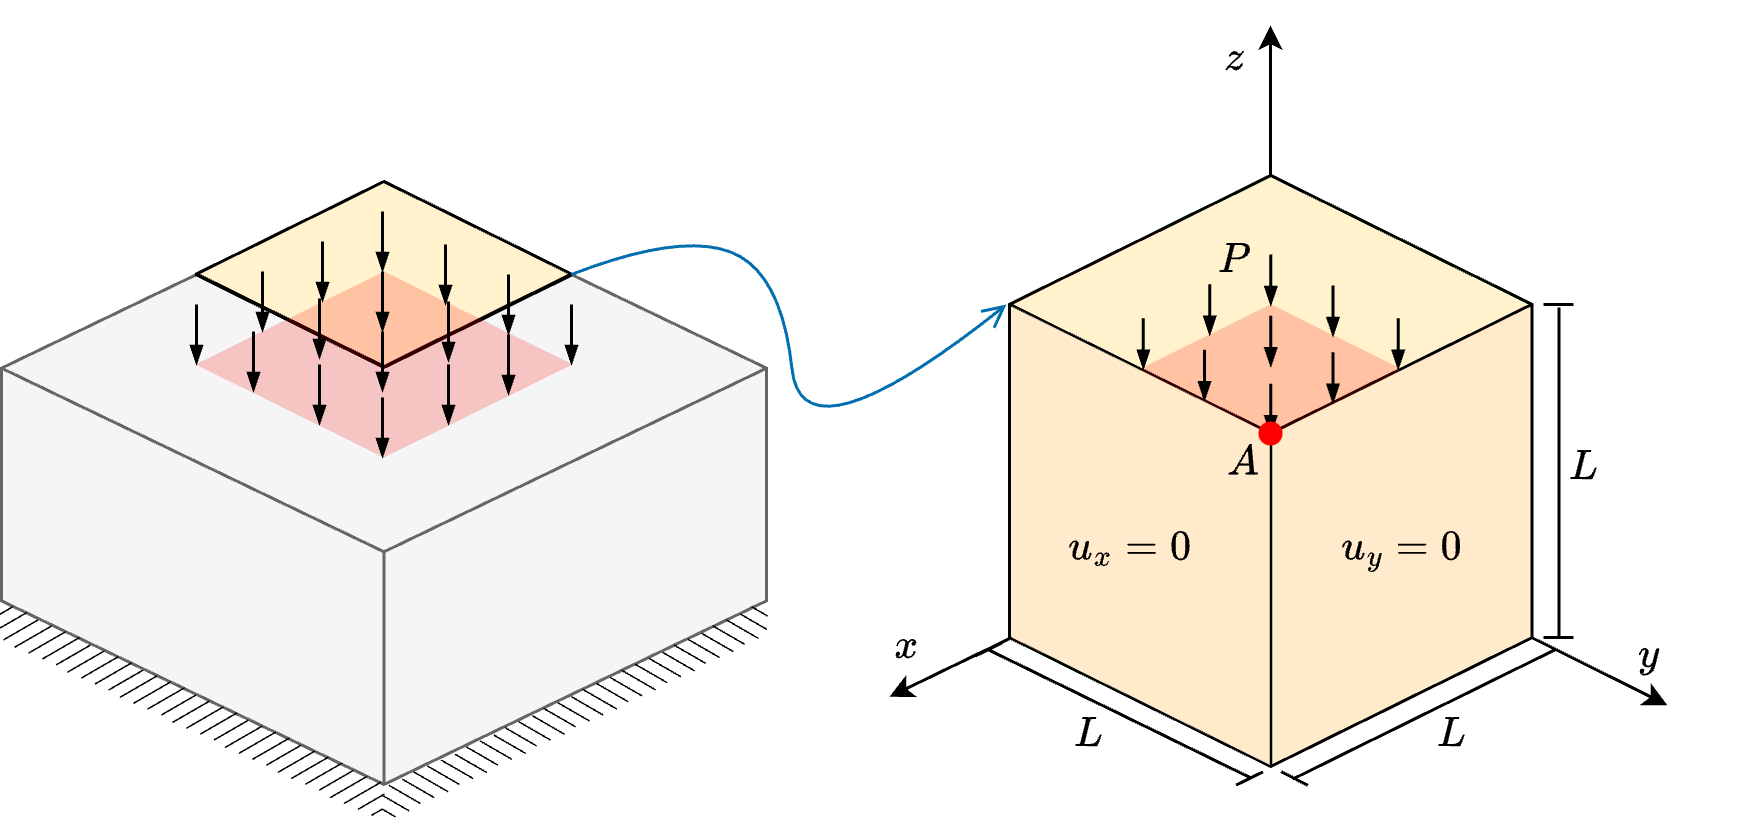
\includegraphics[width=\textwidth]{png/block_model_r1.png}
% 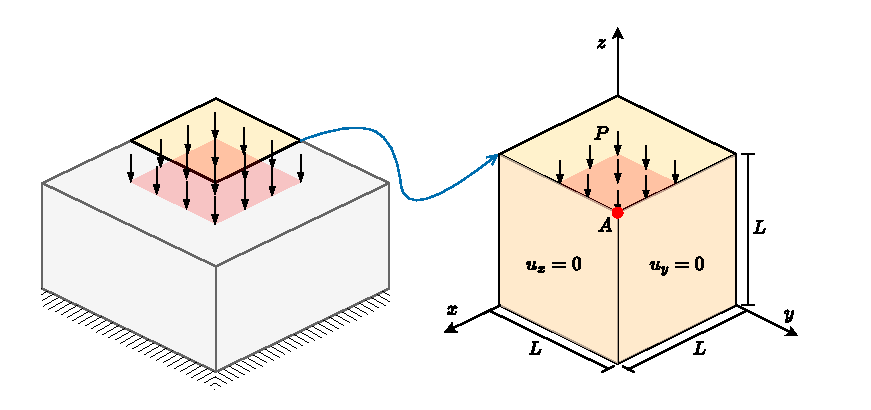
\includegraphics[width=\textwidth]{pdf/block.pdf}
\caption{Illustration of block under compression problem}\label{fg:block_model}
\end{figure}

The convergence properties of the mixed formulations are evaluated by comparing the compression level at point $A$ under  \DIFaddbegin \DIFadd{loading condition $P = 80$}\DIFaddend .
\DIFaddbegin \DIFadd{The 4-node tetrahedron element with the MINI scheme (Tet4--MINI) and the 8-node hexahedron element with piecewise constant pressure formulation (H8P1) are introduced herein as comparison methods.}\DIFaddend
As shown in Figure \ref{fg:block_convergence}, all the results exhibit good convergence behavior across different loading levels.
Figures \ref{fg:block_contour_tet4}, \ref{fg:block_contour_hex8} study the pressure stability of 3D mixed FE-meshfree formulations, Tet4--RK and Hex8--RK, with non-uniform nodal distribution, while the pressure is discretized by linear meshfree approximations with a characterized support size of 1.5. The corresponding results also show the well performance of the proposed optimal constraint ratio $r=r_{opt}$. The mixed formulations with the traditional constraint ratio $r=n_d$ show comparable displacement results, but exhibit significant pressure instability.

\begin{figure}[H]
 \centering
%DIF <  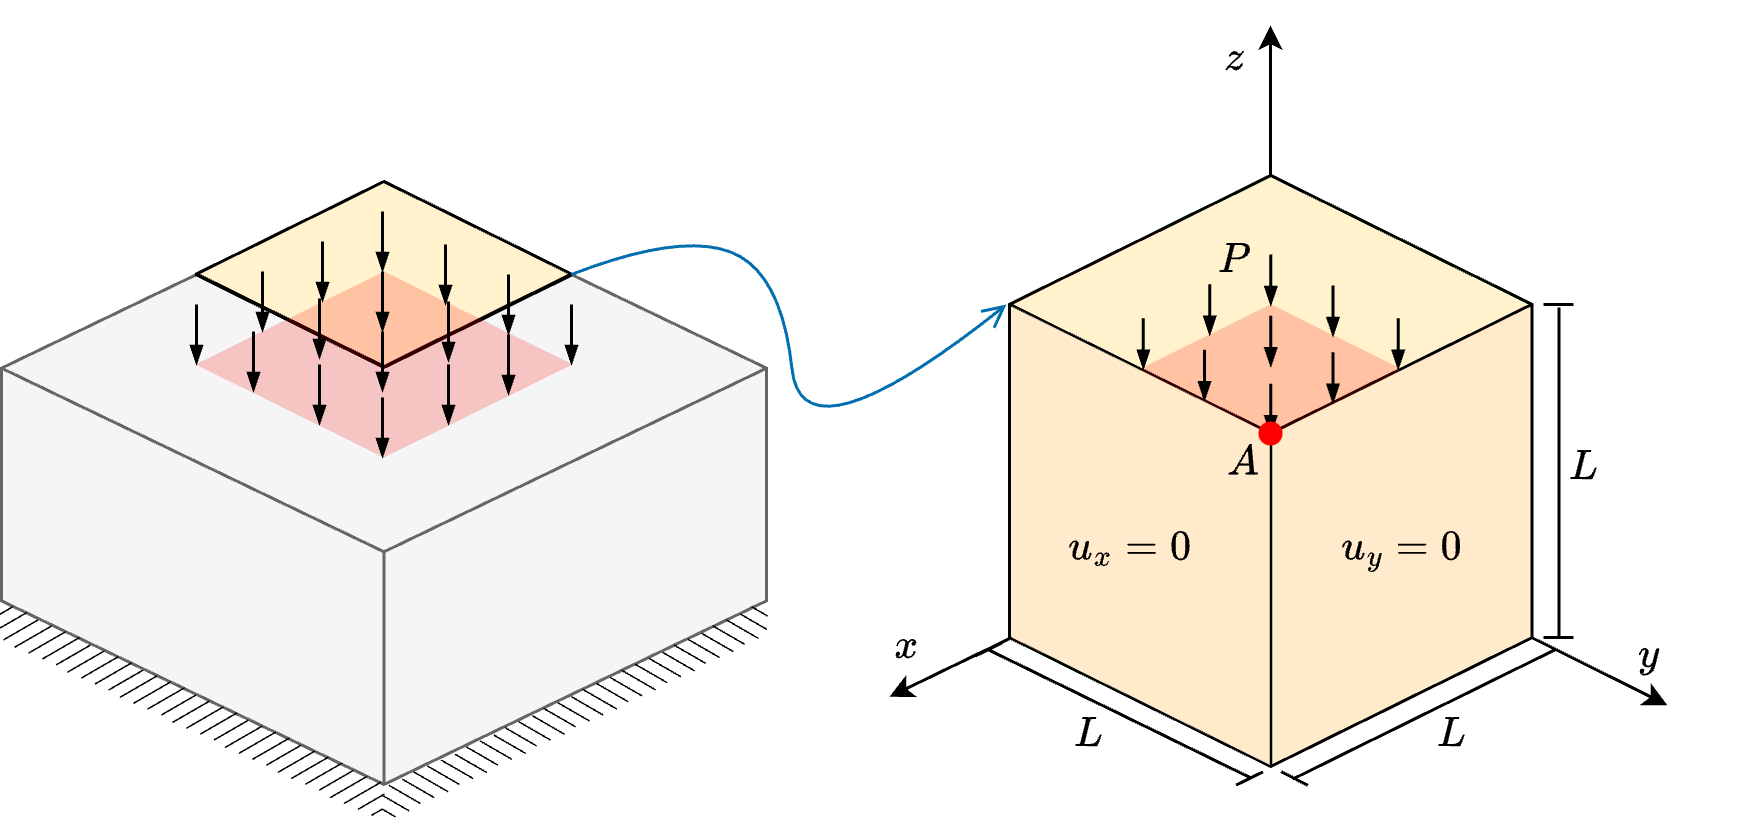
\includegraphics[width=\textwidth]{png/block.png}
 \DIFaddbeginFL 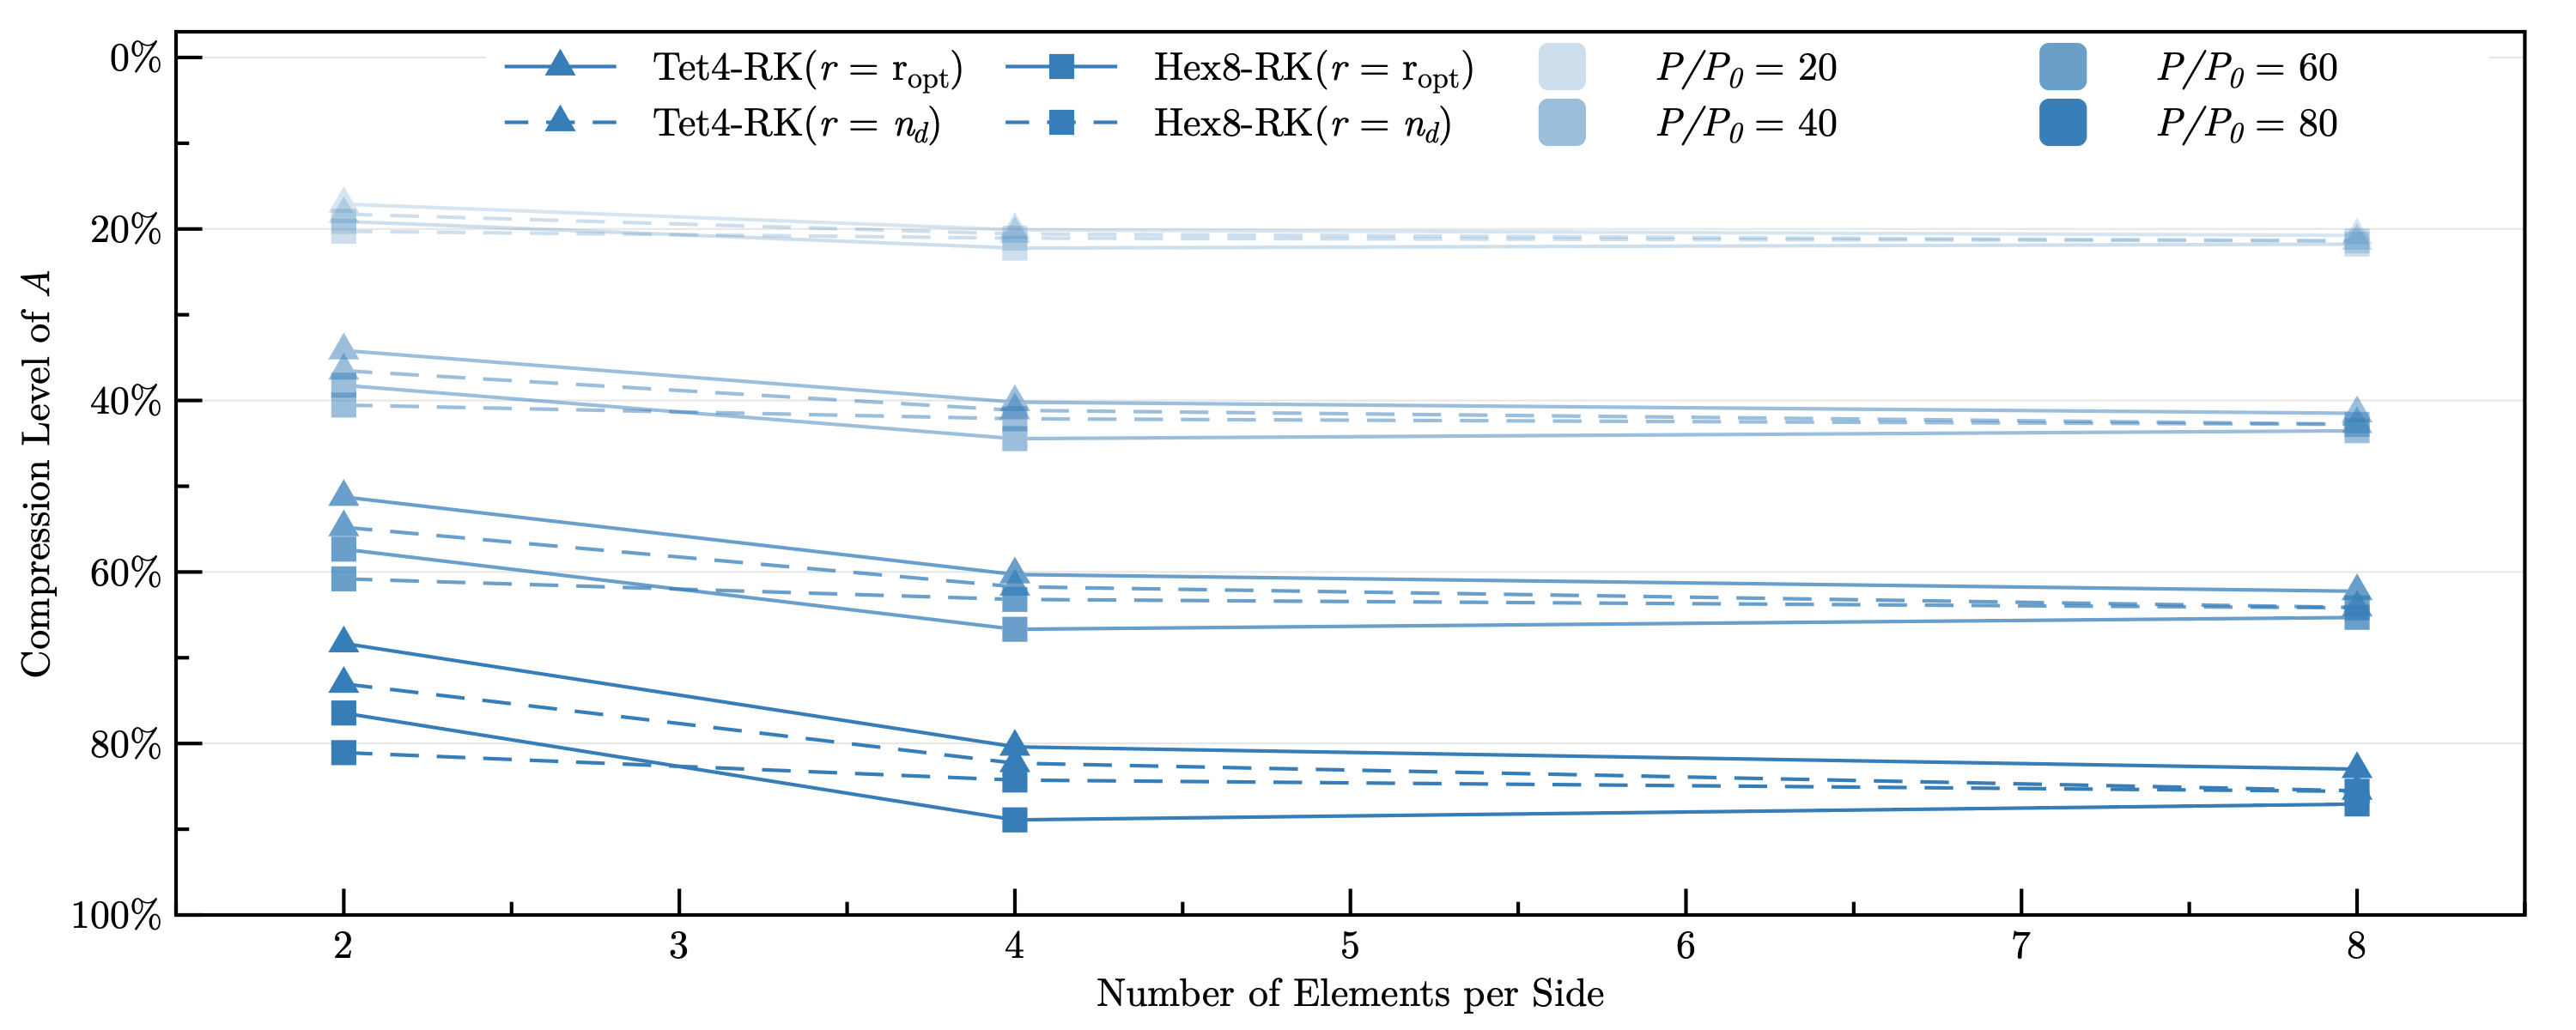
\includegraphics[width=\textwidth]{png/block_convergence.png}
\DIFaddendFL \caption{Convergence comparison of compression level (\%) at point $A$ for block under compression problem}\label{fg:block_convergence}
\end{figure}

\begin{figure}[H]
\centering
\begin{tabular}{c@{\hspace{5pt}}c@{\hspace{5pt}}c@{\hspace{5pt}}c}
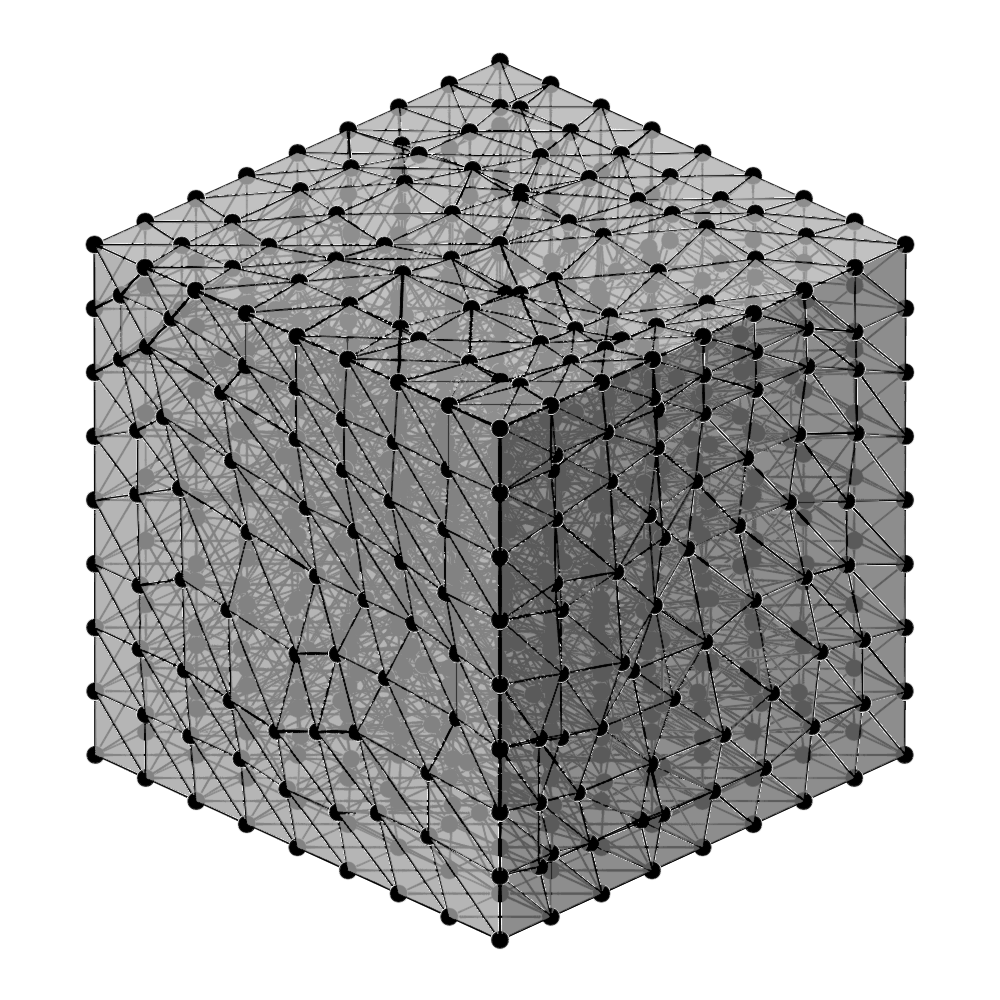
\includegraphics[width=0.3\textwidth]{png/block_tet4_729_msh.png}
& 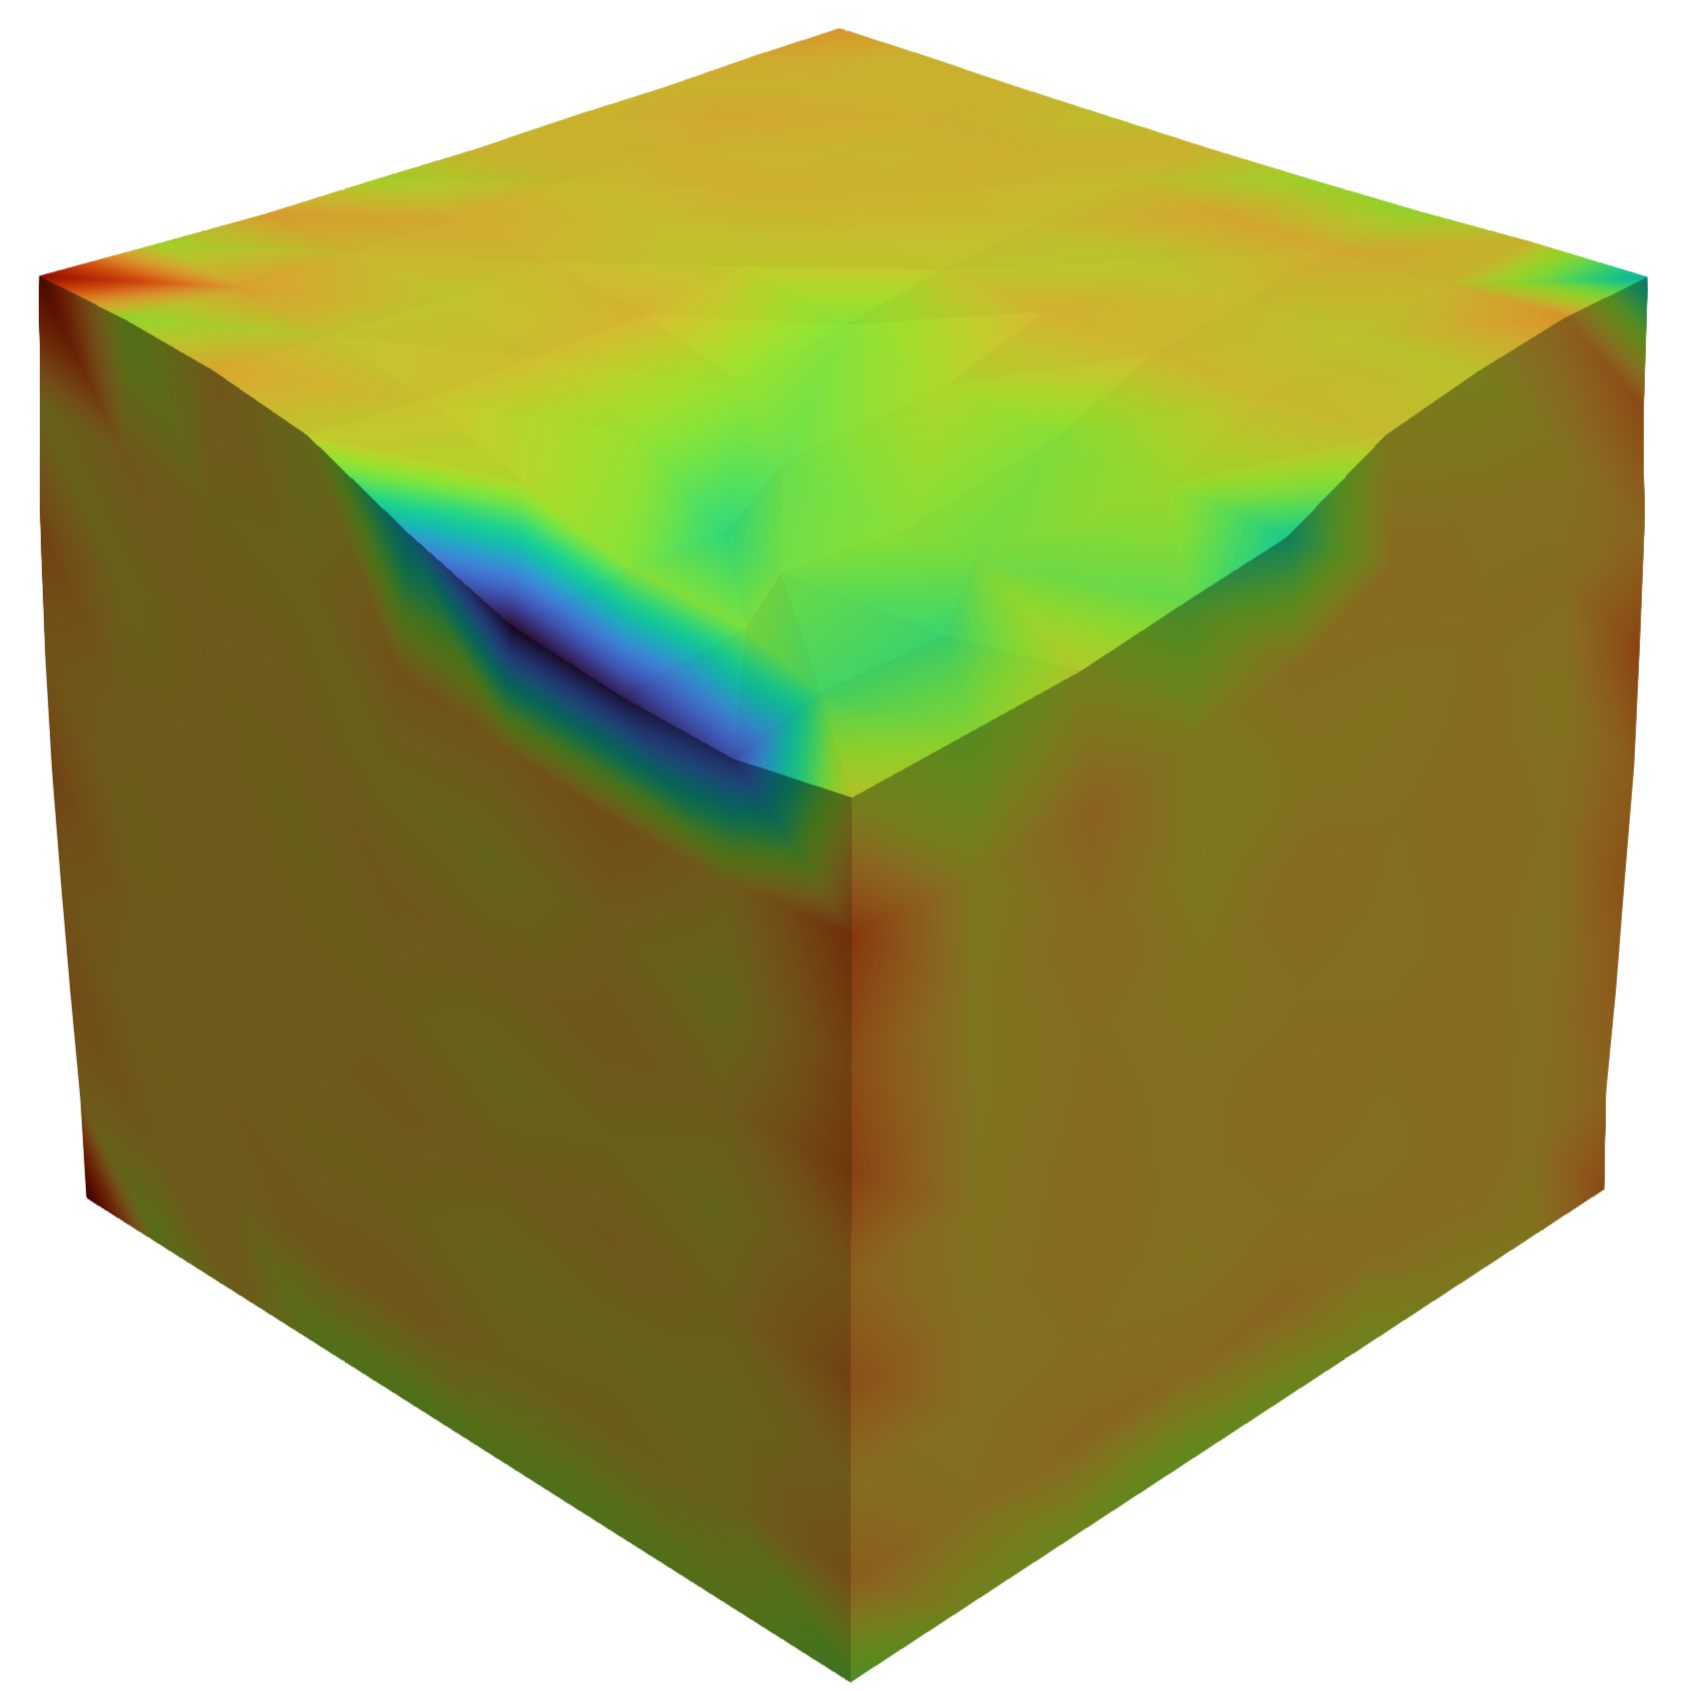
\includegraphics[width=0.3\textwidth]{png/block_tet4_729_729.png}
& 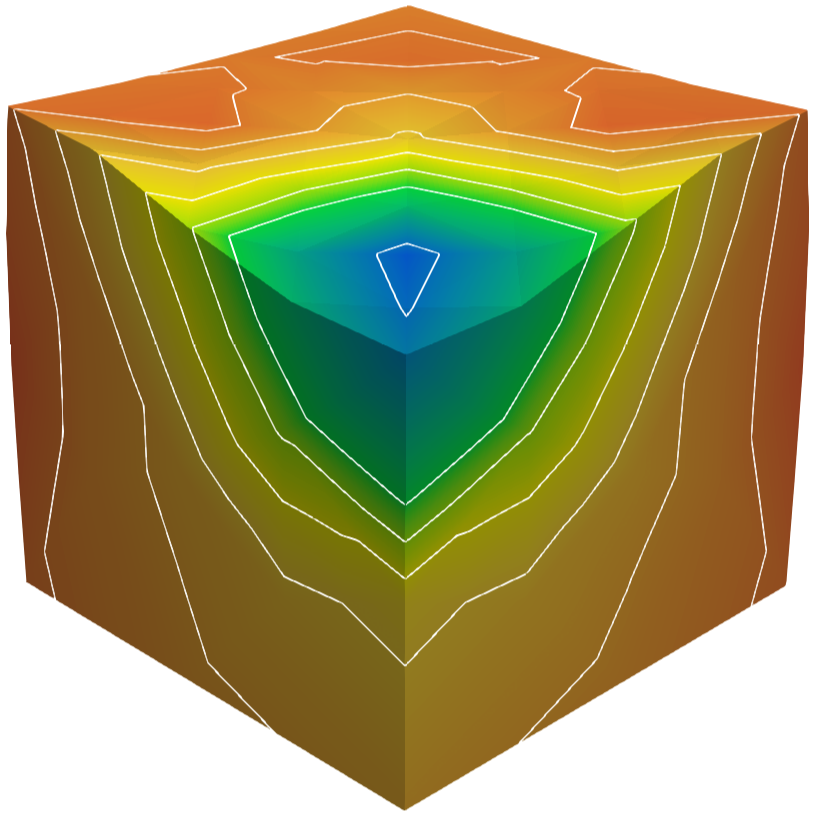
\includegraphics[width=0.3\textwidth]{png/block_tet4_729_125.png}
& 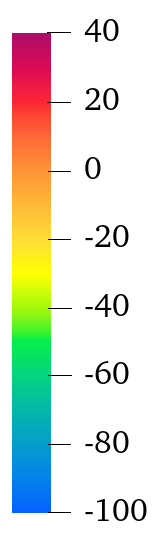
\includegraphics[width=0.1\textwidth]{png/block_legend.png} \\
$n_u = 729$ & $r = n_d$ & $r = r_{opt}$ &
\end{tabular}
\caption{Comparison of pressure contour plots for block under compression problem using Tet4--RK}\label{fg:block_contour_tet4}
\end{figure}

\begin{figure}[H]
\centering
\begin{tabular}{c@{\hspace{5pt}}c@{\hspace{5pt}}c@{\hspace{5pt}}c}
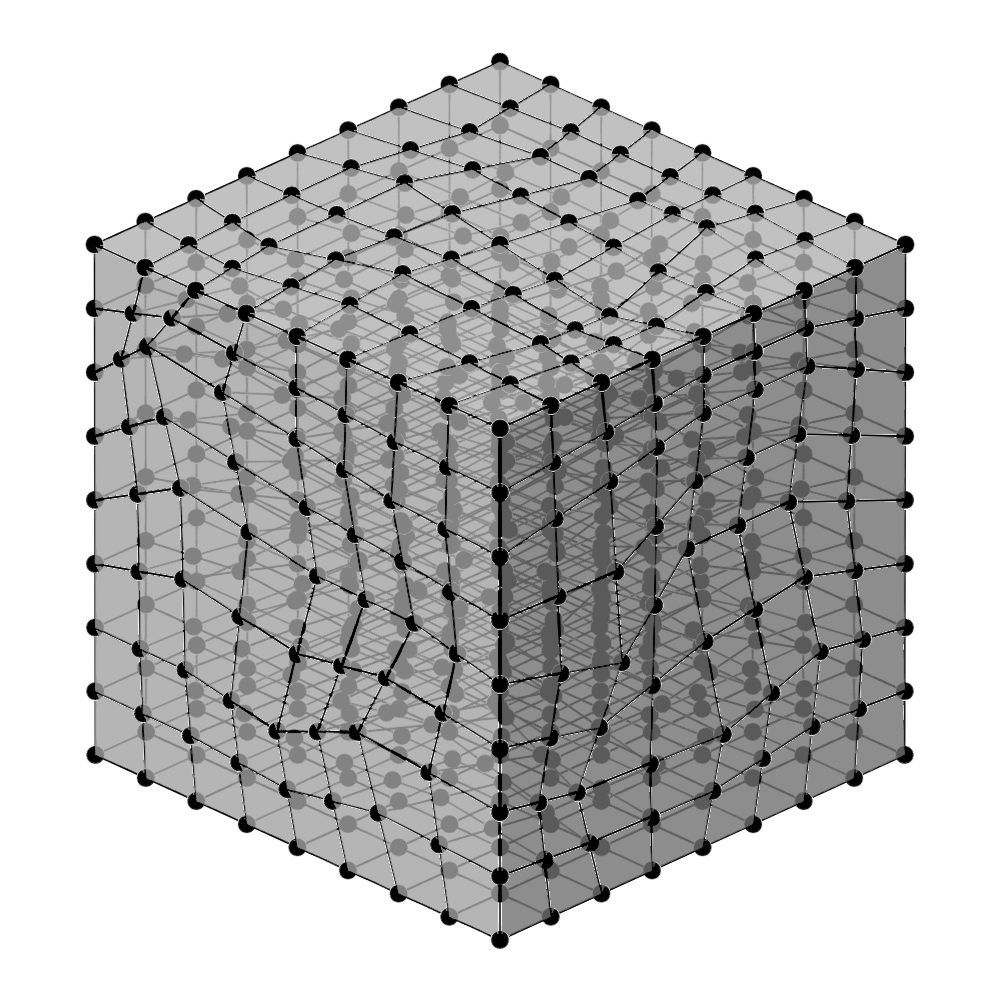
\includegraphics[width=0.3\textwidth]{png/block_hex8_729_msh.png}
& 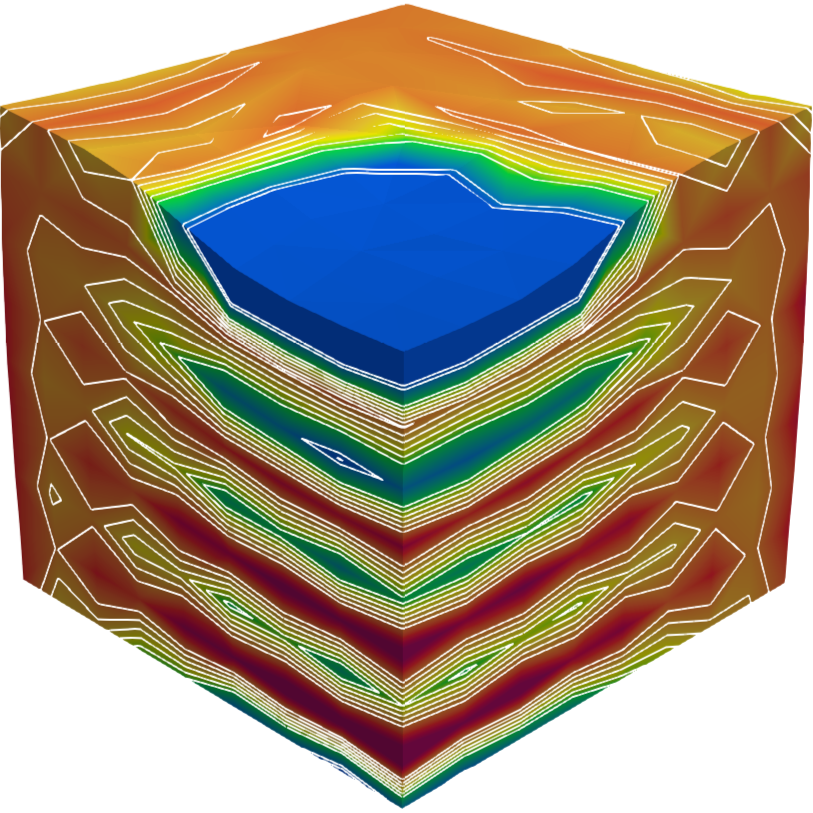
\includegraphics[width=0.3\textwidth]{png/block_hex8_729_729.png}
& 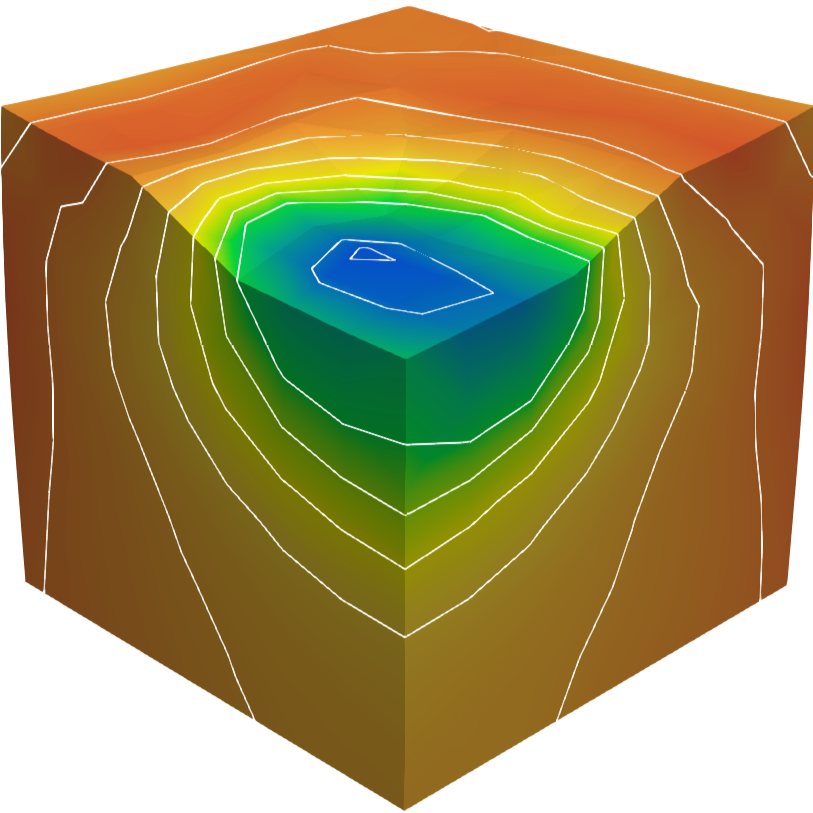
\includegraphics[width=0.3\textwidth]{png/block_hex8_729_125.png}
& 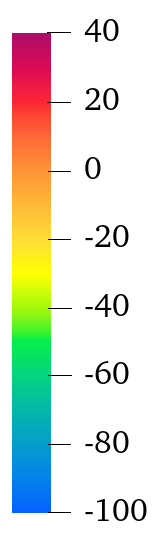
\includegraphics[width=0.1\textwidth]{png/block_legend.png} \\
$n_u = 729$ & $r = n_d$ & $r = r_{opt}$ &
\end{tabular}
\caption{Comparison of pressure contour plots for block under compression problem using Hex8--RK}\label{fg:block_contour_hex8}
\end{figure}


